A system would be useless if it did not operate according to specification.
Therefore, the platform has been thourougly verified through functional tests, performance analysis and example programs.

%==============================================================================%

\section{Functionality}

The functionality of the platform has been verified under normal use conditions with the tests described in Appendix~\ref{app:test-descriptions}.
Each test has a short description and a list of the instructions that are verified given it passes.
Together, the 11 tests cover all system functionality except for fitness, which is designed to be application specific.
The tests are implemented as separate programs, but use a shared test framework.
A full system reset is performed before each test.

All tests are passed for all configurations of the platform that have been implemented, which includes 5x5, 16x16, 32x32, 4x4x4, 8x8x4, 8x8x8, 8x16x8 and 10x10x8 matrix sizes; 5, 6 and 8 type bits; 2, 4, 6, 7 and 8 rules tested in parallel; and 1, 2, 4 and 8 LUT configuration bits.
This proves that the platform is functional and scalable.

\subsection{Fitness}

\TODO

The new DFT module has its own test bench.

It produces slightly different output than before; likely due differences is rounding/expressions between the VHDL and python implementations for generating the twiddle factors.

However, compared to the output of numpy's real fft, the new output is about as precise.

\todo{DFT test results with standard variation / percentage error}
The DFT module is however tested in simulation and compared to the numpy's real fft.

%==============================================================================%

\section{Performance}

As with the previous 3D design, the performance of certain modules scale with the matrix width (X), as they operate on one row of cells at a time.
The main ones are are development, configuration and readback.

\TODO

Closest to Støvnengs CA in 2D:
[rules tested in parallel] = 2.
[lut configuration bits] = 2.

Speed differences:
1/4x config.

Closest to Støvnengs CA in 3D:
[rules tested in parallel] = 2.
[lut configuration bits] = 8.

Speed differences:
4x rsf/live counter.
1/2x config.
1/8x readback.


\todo{best performance}

\subsection{Communication}

\TODO
\tablename~\ref{tab:communication-performance}.

\begin{table}[!ht]
    \renewcommand{\arraystretch}{1.4}
    \centering
    \begin{tabular}{c|c|c}
        \bfseries Mode & \bfseries Latency & \bfseries Throughput \\
        \hline
        Normal & \SI{60.3}{\micro\second} & 2.1 MB/s \\
        Low-latency & \SI{7.3}{\micro\second} & 2.1 MB/s \\
    \end{tabular}
    \caption[Communication performance]{
        Performance of the PCI Express communication unit.
    }
    \label{tab:communication-performance}
\end{table}

\TODO
Likely due to minimum system sleep of around \SI{50}{\micro\second}.

The throughput is not exceptional at around 1\% of the 256MB/s that the PCI Express endpoint block is capable of \cite{ug672}.
This is likely due to the simplistic PIO scheme that require that all transfers go through the CPU.
However, this is not as bad as one would first assume.
Following is a short analysis of the desired throughput for the example program in \figurename~\ref{fig:example-program}.

\begin{figure}[!ht]
\begin{lstlisting}[xleftmargin=0.35\textwidth]
initialize()
while counter[0] != 128:
    develop()
    config()
    step(128)
    send_fitness()
    swap_cell_storage()
    counter[0]++
\end{lstlisting}
\caption[Example program] {
    Example program.
}
\label{fig:example-program}
\end{figure}

Assume the following synthesis parameters:
[LUT Configuration Bits] maximized to 8,
[Rules Tested In Parallel] set to 8,
[Rule Amount] set to 256,
[Fitness] set to DFT with transform size of 128 and 16-bit output values,
and the matrix sized to 10x10x8.

That brings development speed to 3.2 cycles/cell and configuration speed to 1.6 cycles/cell (plus overhead)\footnotemark.
The DFT work in parallel with the rest of the design, therefore adding no further delay, and produces 32 words of data after each 128 steps.
With 800 cells, the time for each loop iteration then becomes a little over $3.2 \cdot 800 + 1.6 \cdot 800 + 128 = 3968$ cycles.
32 words per 3968 cycles at 125 Mhz constitutes around 4 MB/s.
The communication unit can therefore supply 50\% of the desired throughput, which should be acceptable for normal operation.

\footnotetext{
    The execution time of each instruction is detailed in Appendix~\ref{app:isa}.
}

%==============================================================================%

\section{Examples}

\TODO
Stacked demo?

\subsection{Replicator}

Self-replication in CA.
Relatively simple rules can grow a structure of any size given enough development time.

Cyan cells shoot off from the corners to form new loops.

\begin{itemize}
    \item 21 rules and 13 states.
    \item Green goes in circle to form border, red when complete (but not corners).
    \item Cyan detaches from corners to form new circles.
    \item X increases to the right, Y increases downwards.
\end{itemize}

\begin{figure}[!ht]
    \centering
    \begin{subfigure}{0.32\textwidth}
        \centering
        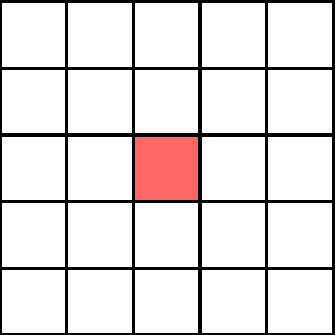
\includegraphics[width=0.9\textwidth]{replicator/00}
        \caption{Step 0}
    \end{subfigure}
    \begin{subfigure}{0.32\textwidth}
        \centering
        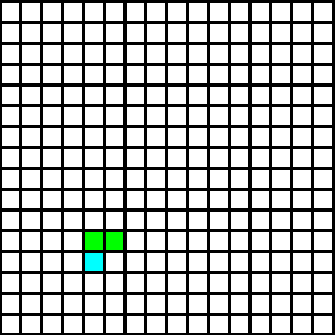
\includegraphics[width=0.9\textwidth]{replicator/01}
        \caption{Step 1}
    \end{subfigure}
    \begin{subfigure}{0.32\textwidth}
        \centering
        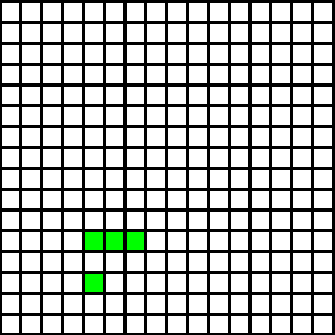
\includegraphics[width=0.9\textwidth]{replicator/02}
        \caption{Step 2}
    \end{subfigure}
    \par\bigskip
    \begin{subfigure}{0.32\textwidth}
        \centering
        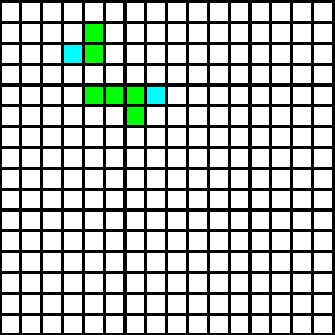
\includegraphics[width=0.9\textwidth]{replicator/03}
        \caption{Step 3}
    \end{subfigure}
    \begin{subfigure}{0.32\textwidth}
        \centering
        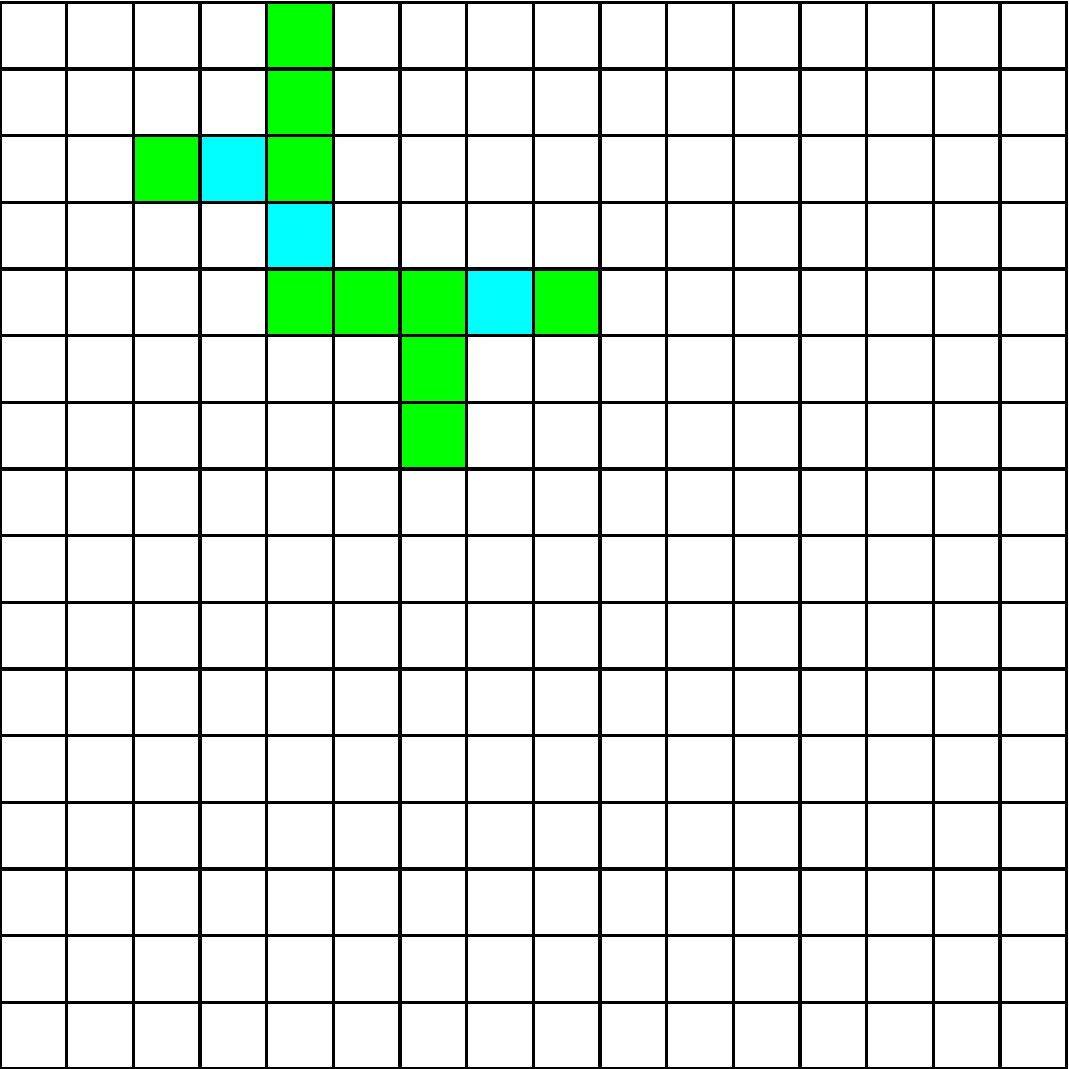
\includegraphics[width=0.9\textwidth]{replicator/04}
        \caption{Step 4}
    \end{subfigure}
    \begin{subfigure}{0.32\textwidth}
        \centering
        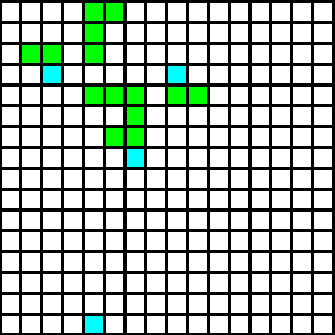
\includegraphics[width=0.9\textwidth]{replicator/05}
        \caption{Step 5}
    \end{subfigure}
    \par\bigskip
    \begin{subfigure}{0.32\textwidth}
        \centering
        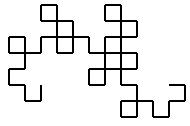
\includegraphics[width=0.9\textwidth]{replicator/06}
        \caption{Step 6}
    \end{subfigure}
    \begin{subfigure}{0.32\textwidth}
        \centering
        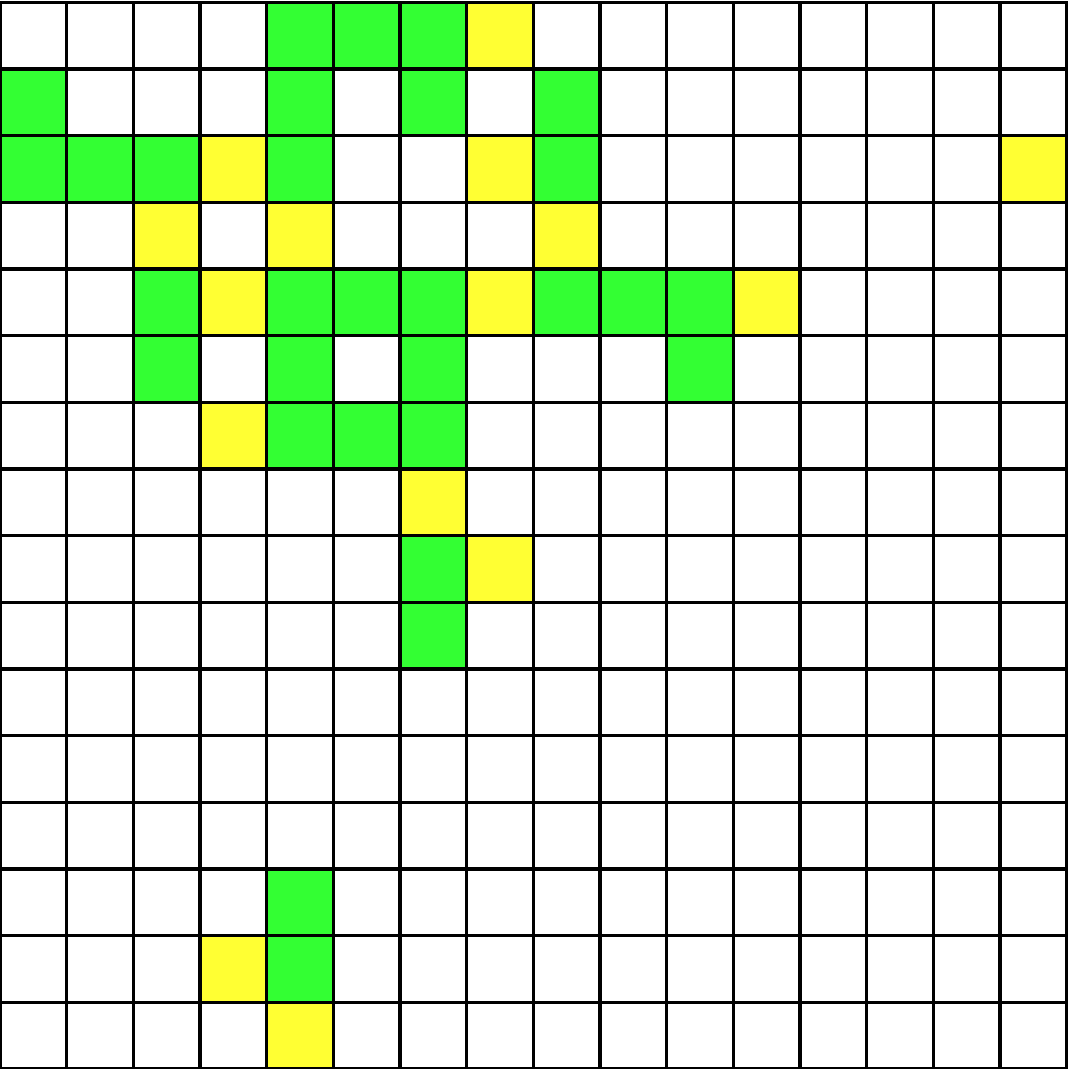
\includegraphics[width=0.9\textwidth]{replicator/07}
        \caption{Step 7}
    \end{subfigure}
    \begin{subfigure}{0.32\textwidth}
        \centering
        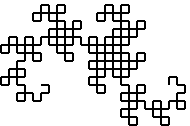
\includegraphics[width=0.9\textwidth]{replicator/08}
        \caption{Step 8}
    \end{subfigure}
    \par\bigskip
    \begin{subfigure}{0.32\textwidth}
        \centering
        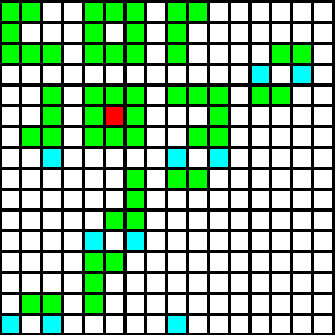
\includegraphics[width=0.9\textwidth]{replicator/09}
        \caption{Step 9}
    \end{subfigure}
    \begin{subfigure}{0.32\textwidth}
        \centering
        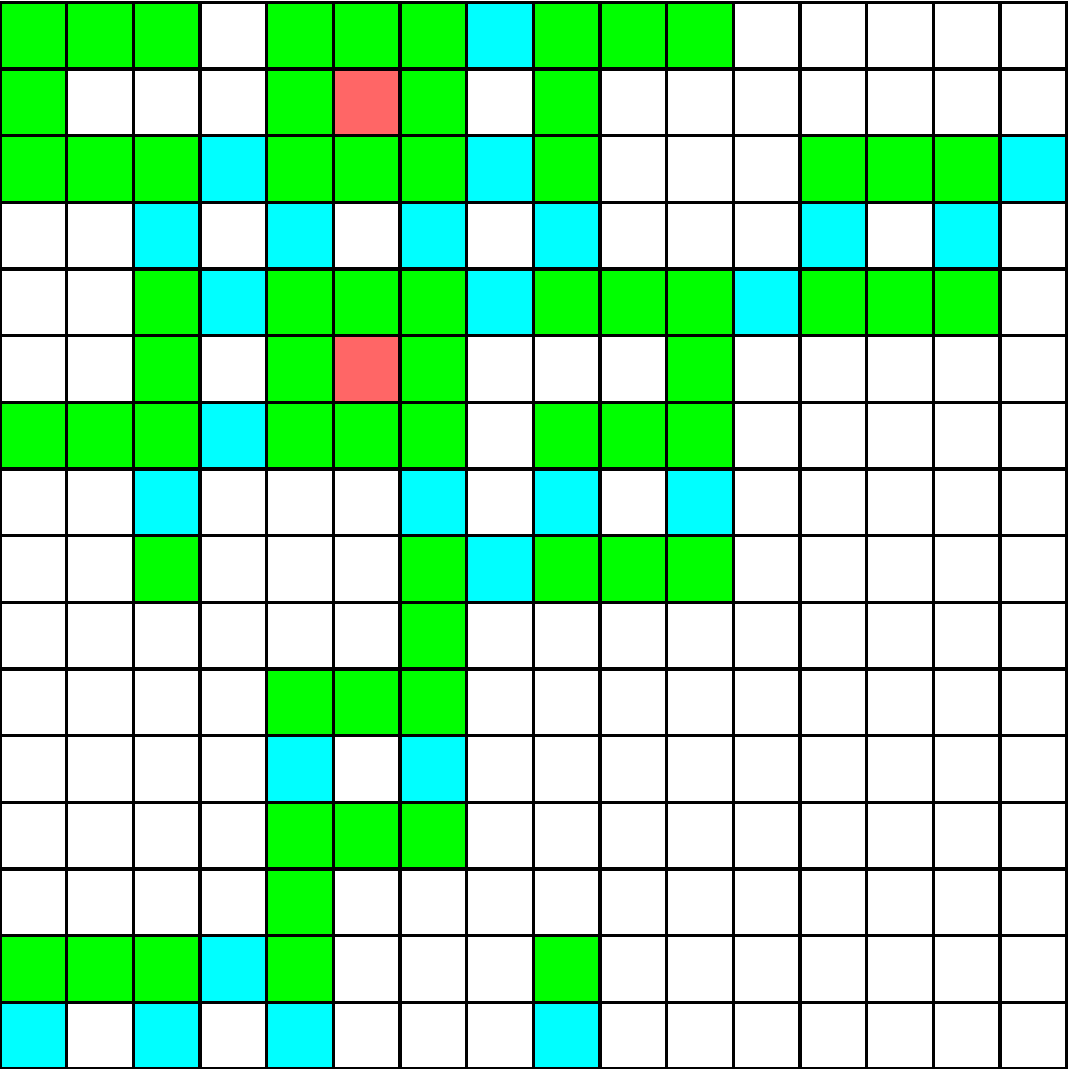
\includegraphics[width=0.9\textwidth]{replicator/10}
        \caption{Step 10}
    \end{subfigure}
    \begin{subfigure}{0.32\textwidth}
        \centering
        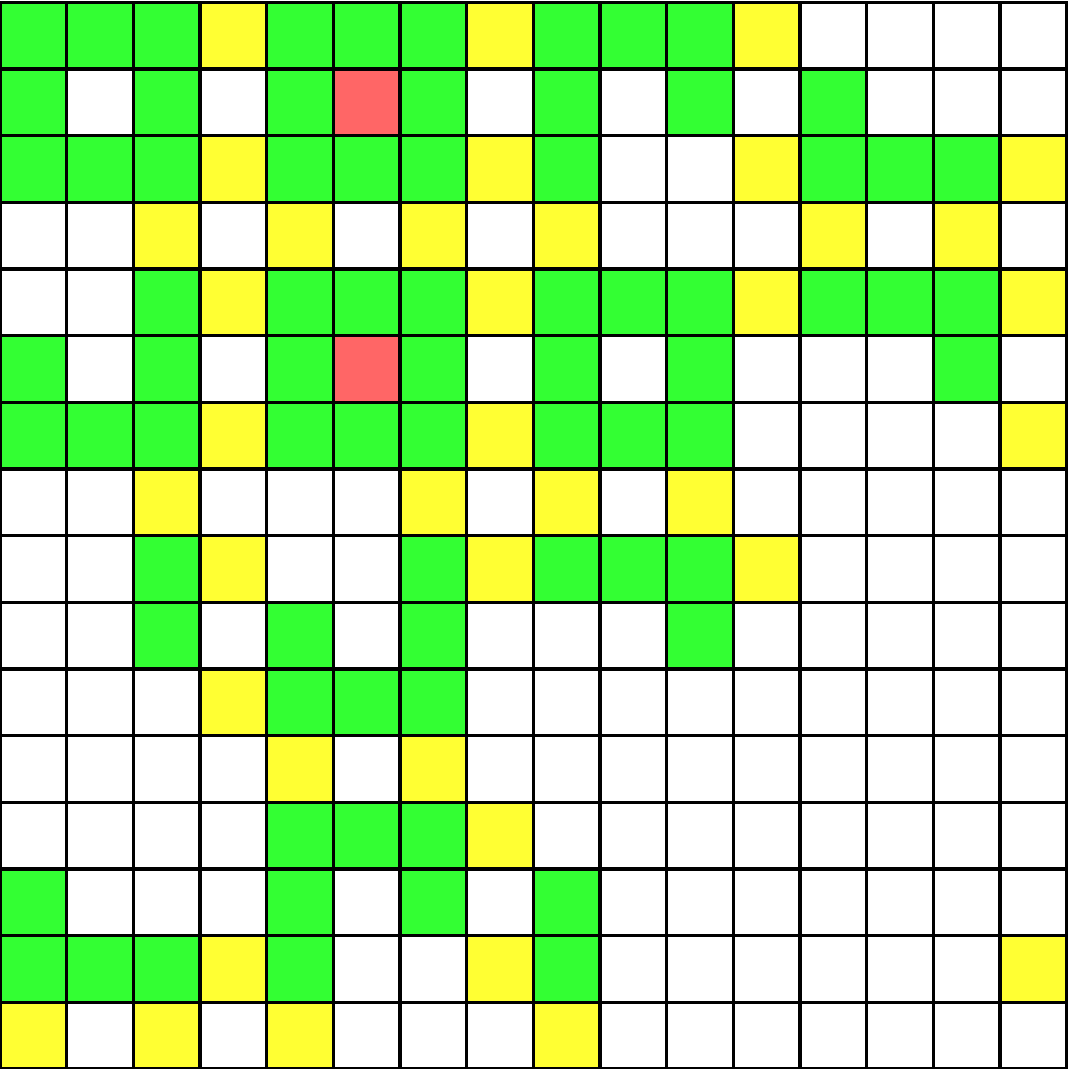
\includegraphics[width=0.9\textwidth]{replicator/11}
        \caption{Step 11}
    \end{subfigure}
\end{figure}

\begin{figure}[!ht]
    \ContinuedFloat
    \centering
    \begin{subfigure}{0.32\textwidth}
        \centering
        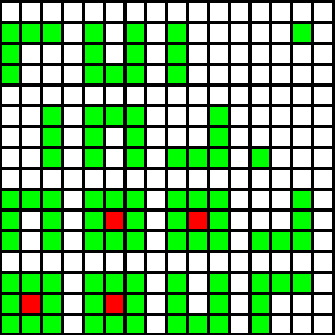
\includegraphics[width=0.9\textwidth]{replicator/12}
        \caption{Step 12}
    \end{subfigure}
    \begin{subfigure}{0.32\textwidth}
        \centering
        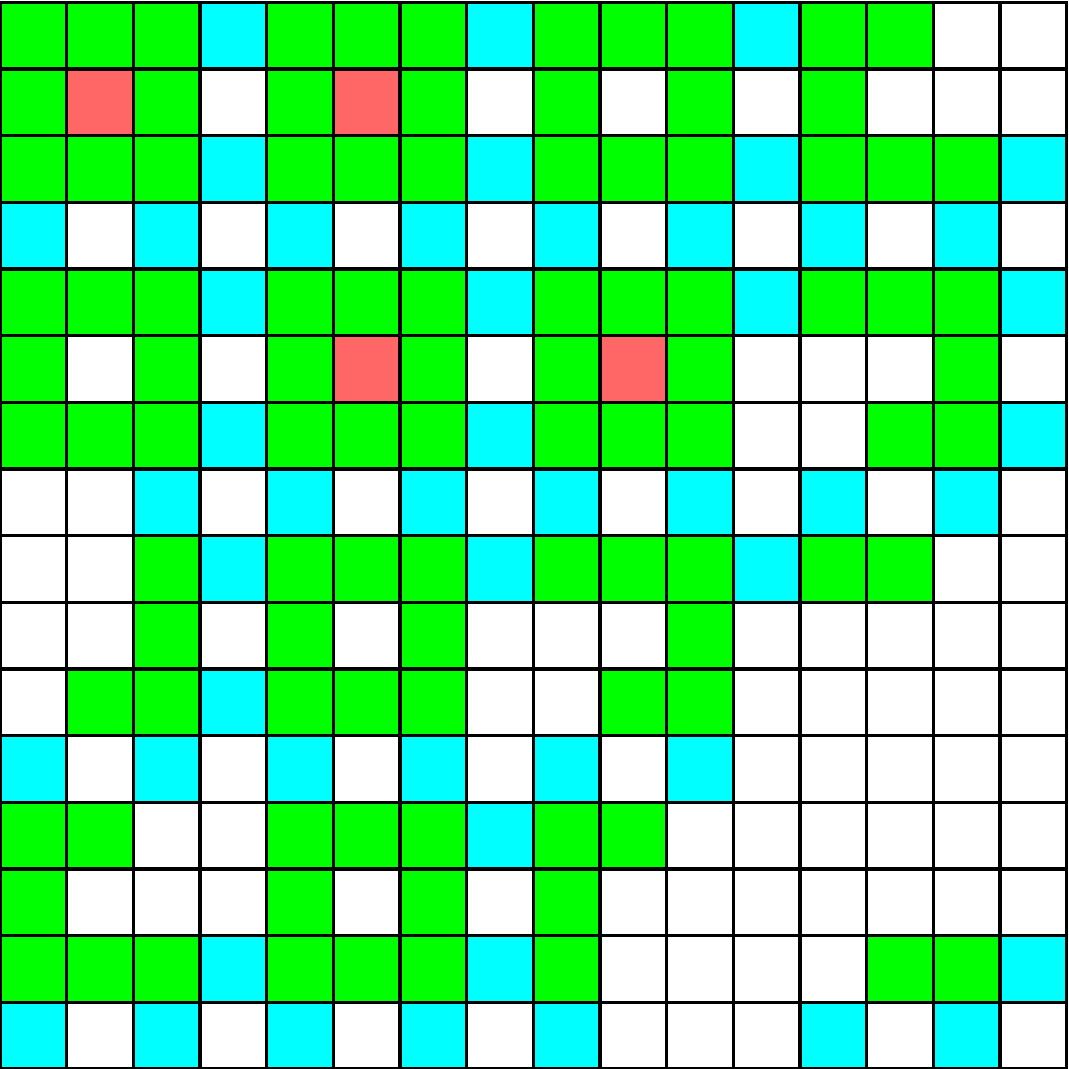
\includegraphics[width=0.9\textwidth]{replicator/13}
        \caption{Step 13}
    \end{subfigure}
    \begin{subfigure}{0.32\textwidth}
        \centering
        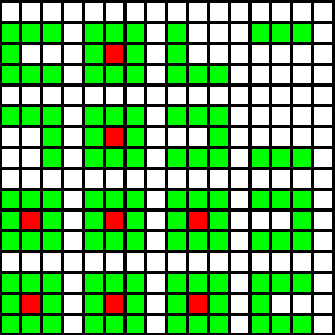
\includegraphics[width=0.9\textwidth]{replicator/14}
        \caption{Step 14}
    \end{subfigure}
    \par\bigskip
    \begin{subfigure}{0.32\textwidth}
        \centering
        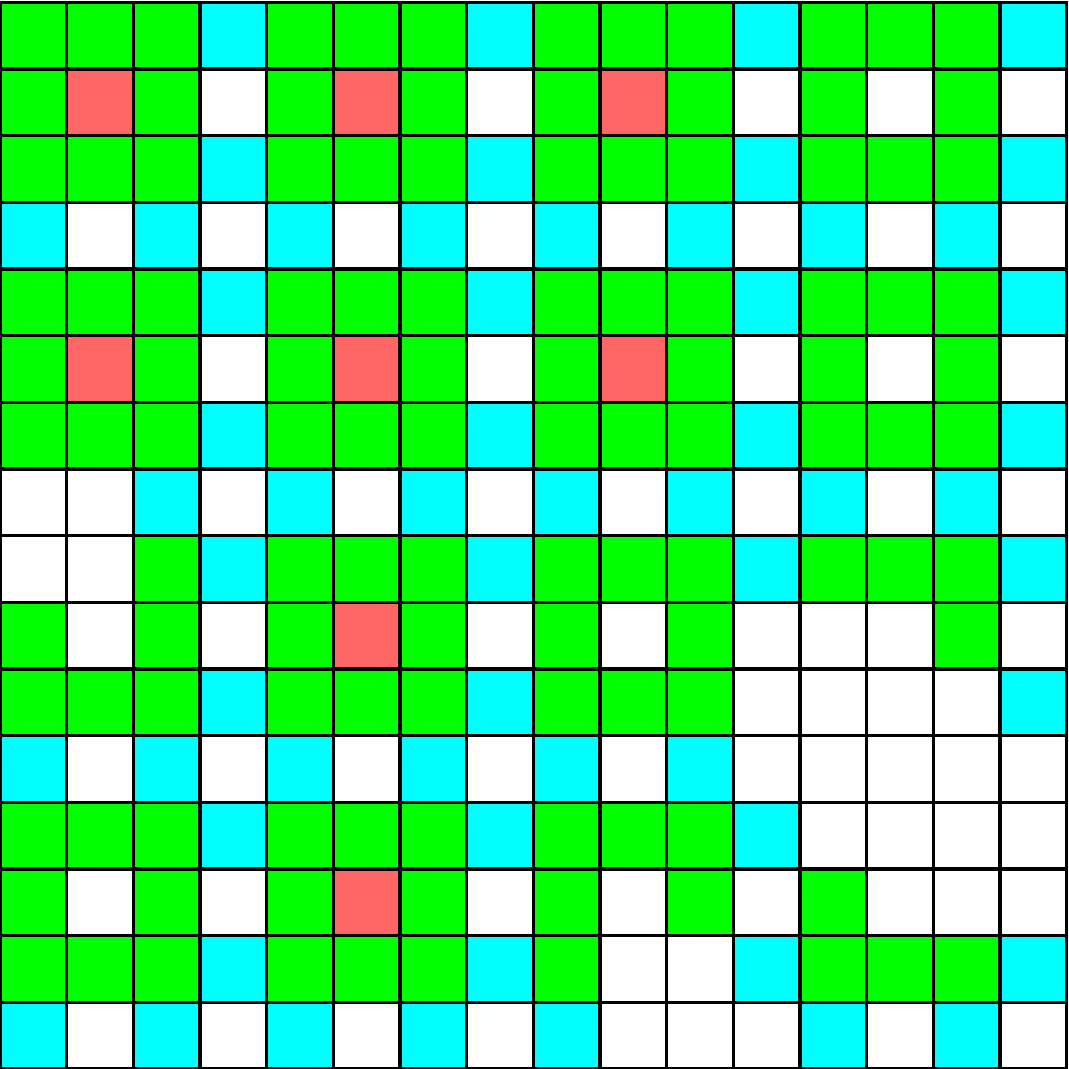
\includegraphics[width=0.9\textwidth]{replicator/15}
        \caption{Step 15}
    \end{subfigure}
    \begin{subfigure}{0.32\textwidth}
        \centering
        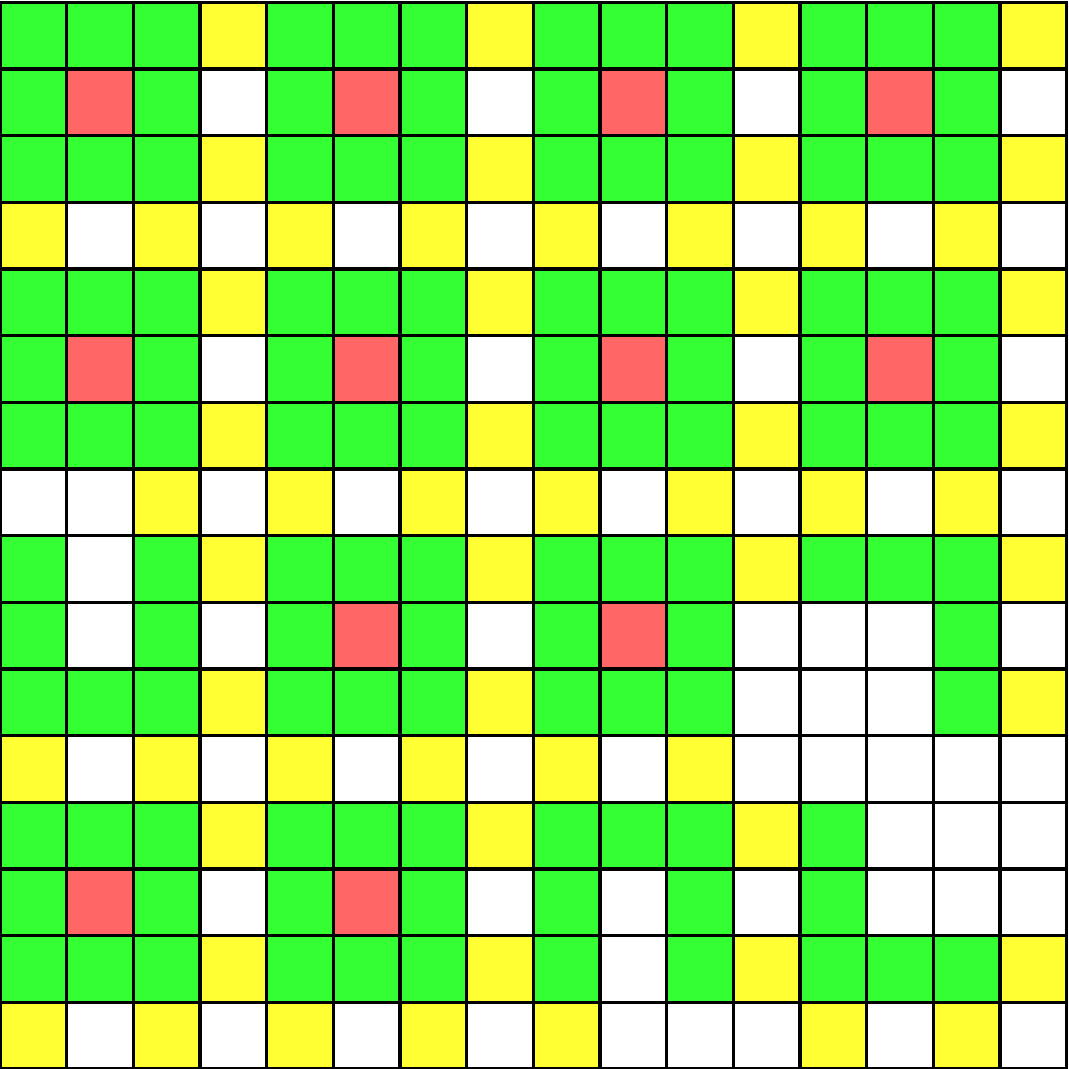
\includegraphics[width=0.9\textwidth]{replicator/16}
        \caption{Step 16}
    \end{subfigure}
    \begin{subfigure}{0.32\textwidth}
        \centering
        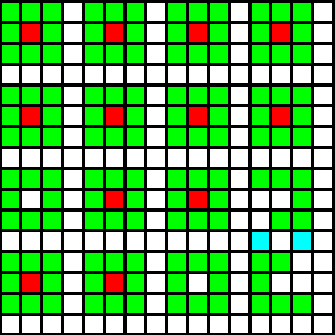
\includegraphics[width=0.9\textwidth]{replicator/17}
        \caption{Step 17}
    \end{subfigure}
    \par\bigskip
    \begin{subfigure}{0.32\textwidth}
        \centering
        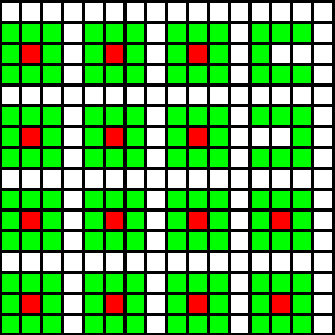
\includegraphics[width=0.9\textwidth]{replicator/18}
        \caption{Step 18}
    \end{subfigure}
    \begin{subfigure}{0.32\textwidth}
        \centering
        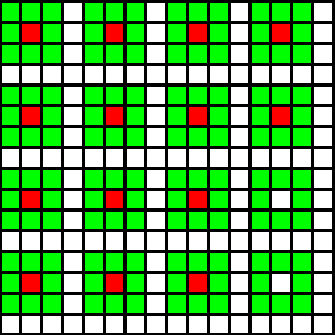
\includegraphics[width=0.9\textwidth]{replicator/19}
        \caption{Step 19}
    \end{subfigure}
    \begin{subfigure}{0.32\textwidth}
        \centering
        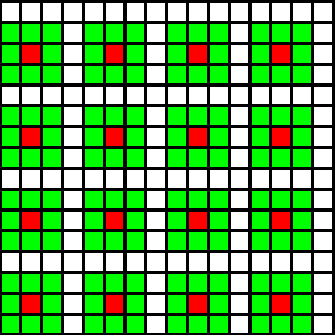
\includegraphics[width=0.9\textwidth]{replicator/20}
        \caption{Step 20}
    \end{subfigure}
    \caption[Replicator] {
        TODO
    }
    \label{fig:replicator}
\end{figure}
